\documentclass[11pt,a4paper,twocolumn]{article}

% ---------- Packages ----------
\usepackage[utf8]{inputenc}    % encoding
\usepackage[T1]{fontenc}
\usepackage[french]{babel}

\usepackage{amsmath, amssymb}  % math
\usepackage{graphicx}          % images
\usepackage{float}             % figure placement
\usepackage{placeins}          % float barriers
\usepackage{hyperref}          % links
\usepackage[margin=1.6cm]{geometry}          % margins
\usepackage{tikz}
\usetikzlibrary{arrows.meta,positioning,calc}
\usepackage{pgfgantt}          % gantt chart
\geometry{margin=2.5cm}

% ---------- Title ----------
\title{Identification des billes projetées d’une mire de calibration\\
pour un système de C-arm}
\author{Jean Faure \and Rayane Bawa \and Clémentine Belaïd \and Alshouni Haiban\\[0.5em]Superviseur : Daniel Elizondo}
\date{\today}

\begin{document}

\twocolumn[
\maketitle
]

\section{Introduction et contexte du projet}

Ce projet s’inscrit dans le cadre d’un projet applicatif en imagerie médicale et chirurgie assistée par robot, en collaboration avec l’entreprise Kyniska Robotics. Kyniska Robotics est une start-up grenobloise fondée en 2024, issue de la fusion de Kat Robotics, Linkx Robotics et OsteSys. Elle développe des solutions de chirurgie robotique, notamment dans les domaines de l’arthrose et des traumatismes du sport.

Dans le contexte de la chirurgie assistée par robot, il est essentiel de connaître avec précision la position des structures osseuses à opérer. Cela nécessite un recalage précis entre des données préopératoires tridimensionnelles, par exemple issues d’un scanner CT, et des images acquises en peropératoire.

\section{Contexte d’imagerie médicale}

Le dispositif étudié dans ce projet est le C-arm, un appareil d’imagerie médicale largement utilisé au bloc opératoire. Le C-arm permet d’acquérir des images radiographiques de haute qualité en temps réel, ce qui est indispensable pour le guidage chirurgical.

\begin{figure}[H]
  \centering
  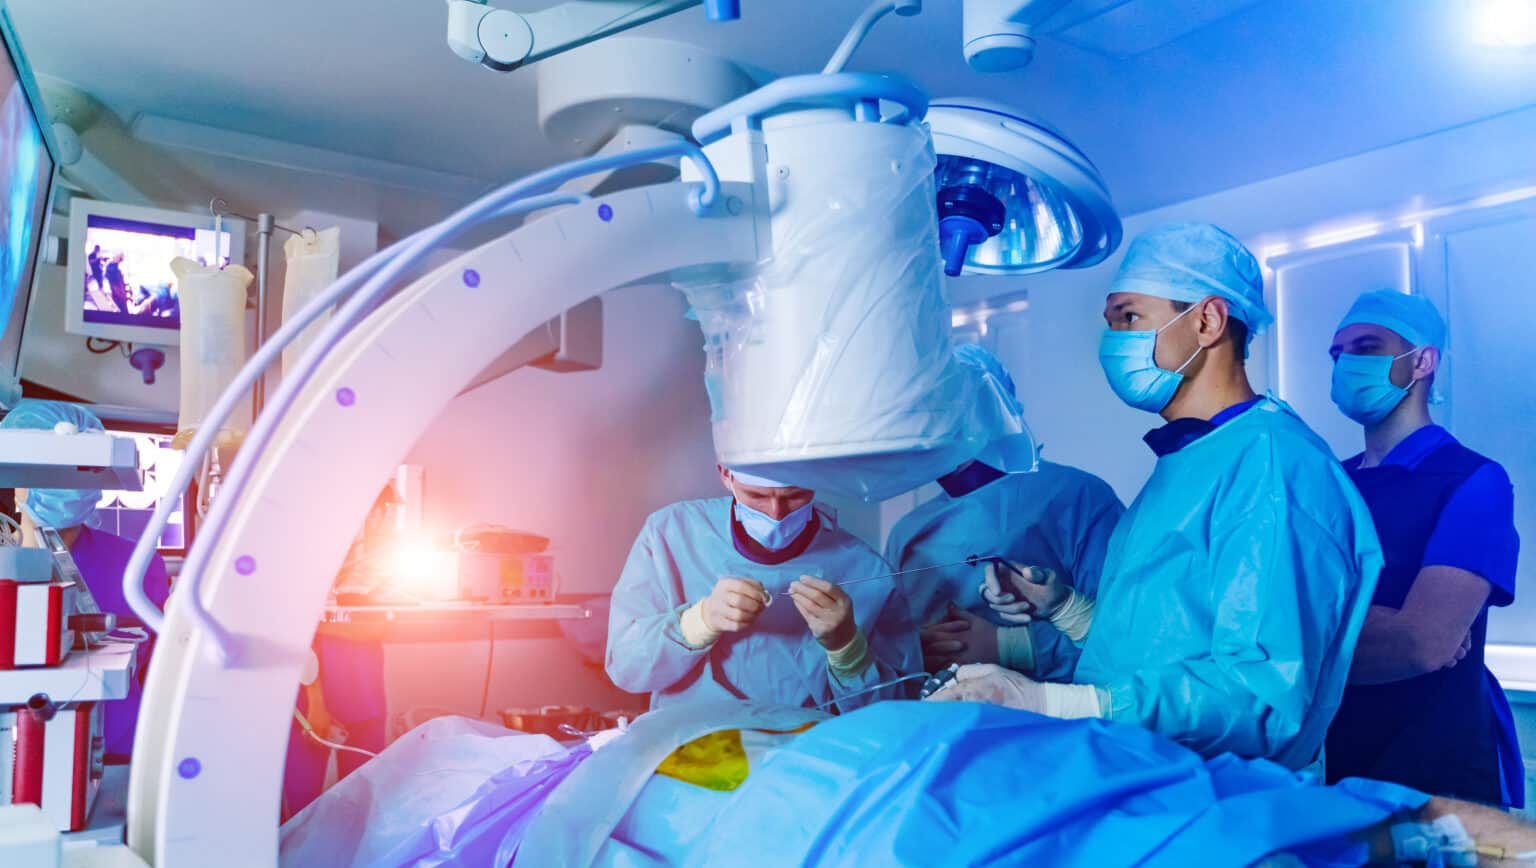
\includegraphics[width=0.95\columnwidth]{figures/photo_C-arm.jpg}
  \caption{Photo C-arm}
\end{figure}

Cependant, les images acquises par le C-arm dépendent fortement de sa position et de son orientation. Pour exploiter correctement ces images à des fins de mesure ou de recalage géométrique, une étape de calibration est nécessaire. Cette calibration repose sur l’utilisation d’une mire de calibration contenant des marqueurs de référence visibles aux rayons X.

\begin{figure}[H]
  \centering
  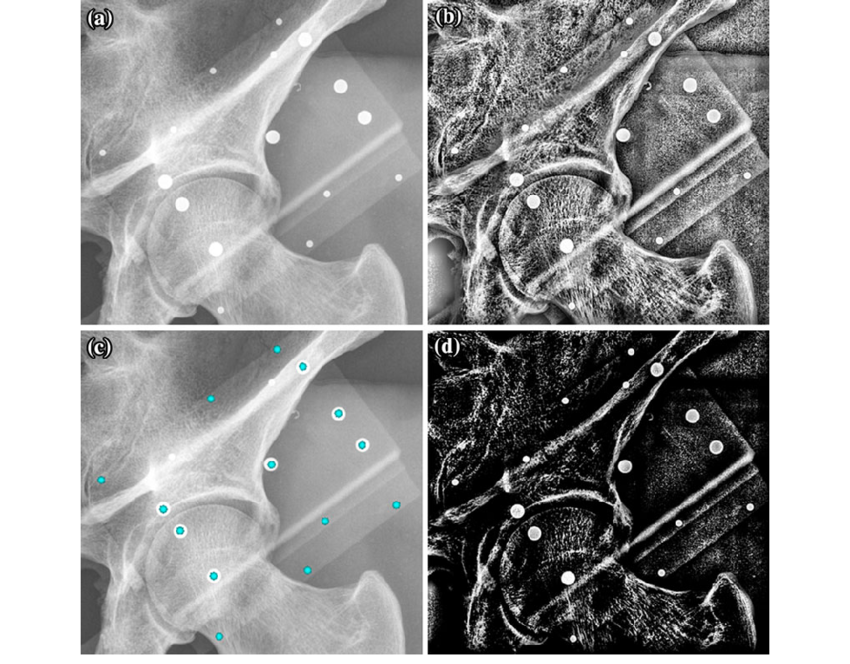
\includegraphics[width=0.95\columnwidth]{figures/image_radio.png}
  \caption{Imagerie médicale avec mire de calibration}
\end{figure}

\section{Mire de calibration et données du problème}

La mire de calibration est un objet tridimensionnel rigide pouvant prendre la forme d’un parallélépipède rectangle ou d’un cône tronqué. Elle contient un ensemble de billes métalliques disposées selon une géométrie connue.

Les caractéristiques typiques de la mire sont les suivantes :
\begin{itemize}
    \item largeur et longueur d’environ 20 cm ;
    \item épaisseur comprise entre 1 et 5 cm ;
    \item nombre de billes compris entre 12 et 30.
\end{itemize}

Ces billes sont visibles sur les images radiographiques et servent de points de référence pour la calibration du système.

\section{Géométrie et mouvements du C-arm}

Le C-arm possède plusieurs degrés de liberté, lui permettant des mouvements de translation et de rotation selon différents axes, tels que la montée et la descente, le déplacement avant et arrière, l’inclinaison et la rotation orbitale.

Ces mouvements modifient la projection perspective de la mire de calibration sur le détecteur 2D. Ainsi, une même mire 3D peut produire des configurations 2D très différentes, ce qui complique l’identification des billes projetées.

\begin{figure}[H]
  \centering
  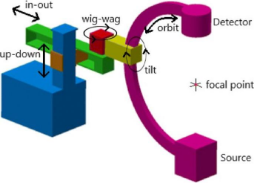
\includegraphics[width=0.9\columnwidth]{figures/schema_C-arm.png}
  \caption{Schéma C-arm}
\end{figure}

\section{Problématique et objectif du projet}

L’objectif principal du projet est l’identification et la numérotation des billes projetées en deux dimensions à partir d’images radiographiques.

Plus précisément, il s’agit de développer un algorithme capable de détecter les billes visibles sur une image 2D et d'associer chaque bille projetée à la bille correspondante dans la mire 3D.

L’algorithme doit être efficace et rapide afin d’être compatible avec une utilisation clinique, tout en restant robuste au bruit et aux artefacts présents dans les images radiographiques.

\section{Méthode connues}

\subsection{Méthode du Birapport et invariance projective}

Le birapport (ou \textit{cross-ratio}) est un invariant fondamental de la géométrie projective, défini pour quatre points distincts et alignés \( A, B, C, D \).

Il est défini par :
\begin{equation}
(A,B;C,D)
= \frac{AC}{BC} \div \frac{AD}{BD}
= \frac{AC \cdot BD}{AD \cdot BC},
\end{equation}
où les distances sont des distances orientées sur la droite support.

Une propriété essentielle du birapport est son invariance par transformation projective. Si \( A', B', C', D' \) désignent les images de \( A, B, C, D \) par une projection, alors :
\begin{equation}
(A,B;C,D) = (A',B';C',D').
\end{equation}
Cette égalité suppose une projection non dégénérée : les quatre points restent distincts et alignés, et la projection n’envoie pas la droite support vers un point à l’infini.

\begin{figure}[H]
  \centering
  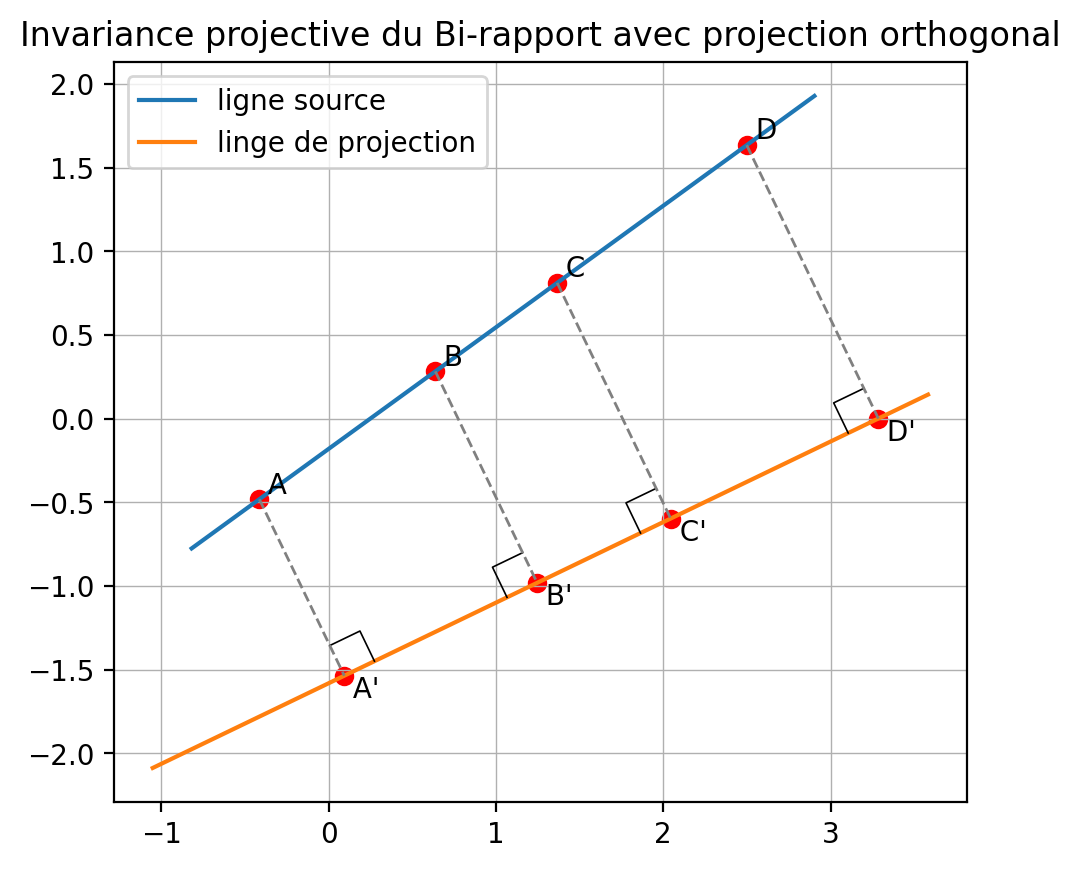
\includegraphics[width=0.9\columnwidth]{figures/proj_ortho.png}
  \caption{Projection orthographique}
\end{figure}

\begin{figure}[H]
  \centering
  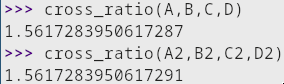
\includegraphics[width=0.9\columnwidth]{figures/cross_ratio.png}
  \caption{invariance du Bi-rapport}
\end{figure}

Cette invariance permet d’utiliser le birapport comme critère local d’identification, en comparant des valeurs de référence connues à celles calculées sur des quadruplets de points observés, à une tolérance près.

\subsection{Méthode de l’enveloppe convexe}

Une seconde approche est basée sur la construction de l’enveloppe convexe des points projetés. Cette méthode exploite la structure géométrique globale du nuage de points.

En identifiant les couches successives de l’enveloppe convexe, il est possible de réduire fortement le nombre de correspondances candidates entre les billes 3D et leurs projections 2D.

\begin{figure}[H]
  \centering
  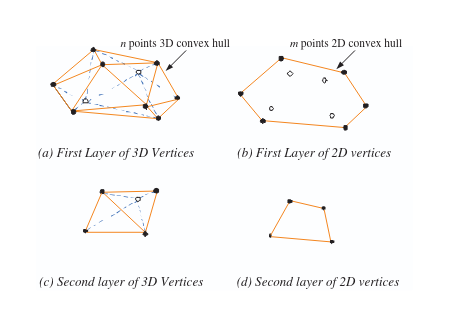
\includegraphics[width=0.9\columnwidth]{figures/convex_hull.png}
  \caption{(a, b) Un parcours de m points dans l'enveloppe convexe de la figure en 3D correspondant à m points dans l'enveloppe convexe de celle en 2D}
\end{figure}

Cependant, cette méthode est sensible au bruit et aux faux positifs, car la présence de points erronés peut modifier la forme de l’enveloppe convexe et entraîner des erreurs d’identification.

\subsection{Comparaison des méthodes}

Les deux méthodes présentent des avantages et des limites complémentaires.  
La méthode de l’enveloppe convexe permet une forte réduction combinatoire, mais elle est peu robuste au bruit.  
À l’inverse, la méthode du birapport est plus robuste au bruit, mais offre une réduction combinatoire plus faible.

Ces caractéristiques suggèrent une utilisation conjointe des deux approches, par exemple en utilisant l’enveloppe convexe pour l’initialisation des correspondances et le birapport pour leur validation.

\section{Organisation et déroulement du projet}

Le projet est structuré autour de trois modules principaux :
\begin{itemize}
    \item un générateur de billes permettant de créer des configurations 3D numérotées et leurs projections 2D, avec ou sans bruit ; (figures 3D, données problème, vérité terrain)
    \item un algorithme d’identification chargé d’associer les billes projetées aux billes de la mire ;
    \item un module de validation permettant d’évaluer les performances de l’algorithme à partir de données de référence.
\end{itemize}

\clearpage
\onecolumn
\shorthandoff{:;!?}
\section{Planification prévisionnelle}

% -- useless LLM filling
% Une planification a été établie afin d’organiser les différentes phases du projet, comprenant la prise en main du problème, l’étude des méthodes existantes, le développement des algorithmes, les tests et la préparation des livrables finaux.

\FloatBarrier
\begin{center}
  \begin{ganttchart}[
    x unit=0.18cm,
    y unit chart=0.8cm,
    vgrid,
    hgrid,
    bar height=0.55,
    bar top shift=0.25,
    group top shift=0.3,
    group height=0.3,
    bar label node/.append style={text width=7cm, align=left, draw, rounded corners=1pt, inner sep=2pt}
  ]{1}{51}
    % 2026-04-20 .. 2026-06-09  (51 days)
    \gantttitle{2026}{51}\\
    \gantttitle{Avril}{11}\gantttitle{Mai}{31}\gantttitle{Juin}{9}\\

    \ganttbar[name=t1]{Approfondir la compréhension du problème}{1}{4} \\
    \ganttbar[name=t2]{Choix de structure}{5}{5} \\
    \ganttbar[name=t3]{Générateur}{8}{10} \\
    \ganttbar[name=t4]{Vérificateur}{8}{10} \\
    \ganttbar[name=t5]{Bi-rapport}{11}{19} \\
    \ganttbar[name=t6]{Enveloppe convexe}{11}{19} \\
    \ganttbar[name=t8]{Amélioration ciblée}{22}{23} \\
    \ganttbar[name=t9]{Développement d'une méthode\\originale}{24}{32} \\
    \ganttbar[name=t11]{Interface graphique}{33}{37} \\
    \ganttbar[name=t12]{Tests}{38}{40} \\
    \ganttbar[name=t14]{Préparation de soutenance}{43}{47} \\
    \ganttbar[name=t15]{Soutenances}{50}{51} \\

    \ganttlink{t1}{t2}
    \ganttlink{t2}{t3}
    \ganttlink{t2}{t4}
    \ganttlink{t3}{t5}
    \ganttlink{t4}{t5}
    \ganttlink{t3}{t6}
    \ganttlink{t4}{t6}
    \ganttlink{t5}{t8}
    \ganttlink{t6}{t8}
    \ganttlink{t8}{t9}
    \ganttlink{t9}{t11}
    \ganttlink{t11}{t12}
    \ganttlink{t12}{t14}
    \ganttlink{t14}{t15}

  \end{ganttchart}
  \par\vspace{0.5em}
  \textbf{Planification prévisionnelle}
\end{center}
\clearpage
\twocolumn
\shorthandon{:;!?}

\subsection{suivi de projet}

Notre groupe prévoit de s’organiser sur les 7 semaines du projet en utilisant Trello pour la planification et le suivi des tâches. Des réunions de groupe régulières sont envisagées afin de faire le point sur l’avancement et d’ajuster l’organisation si nécessaire.

\subsection{organisation du groupe}

Il est prévu de donner à l’encadrant un accès au dépôt Git. Un rapport hebdomadaire synthétique sera rédigé et des rendez-vous pourront être organisés au besoin pour discuter des points techniques ou organisationnels.

\section{Outils et technologies utilisés}

Les outils de développement utilisés dans le cadre du projet sont :
\begin{itemize}
    \item les langages C++ ou Python ;
    \item  OpenGL pour la modélisation 3D ;
    \item git (dépot github)
\end{itemize}

Les outils d'organisation utilisés dans le cadre du projet sont :
\begin{itemize}
    \item Trello ;
    \item Gantt ;
    \item Whatsapp ;
\end{itemize}


\end{document}
